\documentclass[12pt,a4paper]{article}
\usepackage{iftex}
\ifXeTeX
  \usepackage{fontspec}
  \IfFontExistsTF{Times New Roman}{\setmainfont{Times New Roman}}{\setmainfont{TeX Gyre Termes}}
\else\ifLuaTeX
  \usepackage{fontspec}
  \IfFontExistsTF{Times New Roman}{\setmainfont{Times New Roman}}{\setmainfont{TeX Gyre Termes}}
\else
  \usepackage[T1]{fontenc}\usepackage[utf8]{inputenc}\usepackage{mathptmx}
\fi\fi
\usepackage{textcomp}
\usepackage[margin=2.5cm]{geometry}
\usepackage{graphicx,booktabs,tabularx,xltabular,enumitem,xcolor,caption,amsmath}
\definecolor{linkblue}{HTML}{1F4E8C}
\IfFileExists{xurl.sty}{\usepackage{xurl}}{}
\usepackage[colorlinks=true,linkcolor=linkblue,urlcolor=linkblue,citecolor=linkblue]{hyperref}\urlstyle{same}
\definecolor{boxbg}{HTML}{F3EEE4}
\captionsetup{labelformat=empty,justification=raggedright,singlelinecheck=false,skip=4pt}
\setlength{\parindent}{0pt}\setlength{\parskip}{6pt}\setlength{\emergencystretch}{3em}
\renewcommand{\arraystretch}{1.25}
\usepackage{titlesec}
\titleformat{\section}{\large\bfseries}{}{0pt}{}
\titleformat{\subsection}{\normalsize\bfseries}{}{0pt}{}
\titlespacing*{\section}{0pt}{14pt}{4pt}
\titlespacing*{\subsection}{0pt}{10pt}{2pt}
\usepackage{fancyhdr}\pagestyle{fancy}\fancyhf{}\renewcommand{\headrulewidth}{0pt}
\fancyfoot[C]{\small\thepage}\fancyhead[R]{\small\textsc{Space Shock}}
\begin{document}
{\raggedright{\LARGE\bfseries When Rockets Fail: Financial Contagion and Competitive Effects in the Space Industry\par}\vspace{6pt}{\large Evidence from publicly listed launch providers: stock market reactions to orbital launch failures, 2000 to 2026.\par}\vspace{8pt}{\normalsize Nahian Ibnat \textperiodcentered{} Nov 2026\par}{\small Interactive version: \url{https://nahianibnat-2000.github.io/space-shock/}\par}}
\vspace{6pt}
\begin{abstract}
\noindent This paper asks how equity markets react when an orbital launch fails, both for the company that built the rocket and for its publicly listed competitors. Using 138 orbital launch failures from 2000 to 2026 (GCAT) and a market-model event study with a prespecified test, it finds that in the 4 failures with a listed maker (2 firms) the maker's two-day cumulative abnormal return was between \textminus{}8.8\% and \textminus{}16.3\%, each case with a 95\% interval excluding zero. Across 24 failures with listed competitors (42 stock reactions, 3 firms, 22 independent events), the equal-weighted average two-day cumulative abnormal return is +0.28\% (95\% cluster-robust interval \textminus{}1.62\% to +2.18\%; cluster-robust p = 0.76); the prespecified standardized test (Boehmer-Musumeci-Poulsen with a Kolari-Pynnönen adjustment) gives p = 0.40. The evidence therefore establishes neither systematic contagion nor systematic competitive gains among these firms, and it does not show the effect is negligible: average effects of about 2.7\% in either direction would usually go undetected. The sign of the estimate changes with how events and firms are weighted, and every independent event involves Avio SpA. The study is a small-sample study of listed firms, not an estimate for the launch industry as a whole.
\end{abstract}

\emph{Keywords:} event study; industry spillovers; contagion; competitive effects; launch failures

\emph{JEL:} G14, L13

\section*{\hypertarget{s1}{}1. Introduction}
When a rocket fails, the company that built it loses the rocket, often a customer's satellite, and usually several months of flights while engineers find the cause. In the United States, for example, a licensed launch operator must investigate the root cause of any mishap, report the results to the regulator, and put in place measures that stop it from happening again (\hyperlink{ref-faa2021}{Federal Aviation Administration, 2021}). The effect of the failure on the maker's competitors is much less clear, and it is the main question of this paper.

Economists describe two opposite ways in which bad news at one firm can move the share prices of other firms in the same industry (\hyperlink{ref-lang1992}{Lang \& Stulz, 1992}). The first is contagion: investors read the failure as news about the whole industry, for example that rockets are riskier than they thought or that rules will become stricter, and they lower their estimate of the value of every firm in it. The second is the competitive effect: investors expect customers to move their satellites to providers whose rockets still work, so the competitors gain. The two channels push share prices in opposite directions, so theory alone cannot say which one is larger. Only data can.

The question matters more now than it did a decade ago, because launch companies have become a larger part of public stock markets. In June 2026 SpaceX began trading on the Nasdaq after raising about \$75 billion, the largest initial public offering on record (\hyperlink{ref-euronews2026}{“SpaceX Makes Its Nasdaq Debut,” 2026}). When more launch firms are listed, more investors hold shares whose value depends on how the market prices launch risk, both the risk of a firm's own rockets and the risk of its competitors' rockets. Whether a failure at one provider moves the shares of the others matters for how investors diversify, for how they value new listings, and for how firms and regulators think about the industry's exposure to a single accident.

Earlier work has answered the same question for other industries. Studies of bankruptcies (\hyperlink{ref-lang1992}{Lang \& Stulz, 1992}), bank failures (\hyperlink{ref-aharony1983}{Aharony \& Swary, 1983}), product recalls (\hyperlink{ref-jarrell1985}{Jarrell \& Peltzman, 1985}) and air crashes (\hyperlink{ref-bosch1998}{Bosch et al., 1998}; \hyperlink{ref-chance1987}{Chance \& Ferris, 1987}) show that bad news at one firm often moves the share prices of its competitors, and that the direction depends on the industry. For spaceflight, the evidence comes mainly from a single event, the loss of the space shuttle Challenger in 1986 (\hyperlink{ref-blose1996}{Blose et al., 1996}; \hyperlink{ref-maloney2003}{Maloney \& Mulherin, 2003}), and from studies of satellite operators, who are the launch firms' customers rather than their competitors (\hyperlink{ref-abramov2015}{Abramov \& Kiang, 2015}). To the author's knowledge, no study has measured how listed launch providers react to the failures of their competitors across many events.

This paper fills that gap with an event study of orbital launch failures from 2000 to 2026. An event study measures how much a share price moves on and just after a specific piece of news, beyond what the general movement of the market on those days would predict (\hyperlink{ref-mackinlay1997}{MacKinlay, 1997}). Launch failures suit the method well. They happen at a known time, they are usually broadcast live, and they are not caused by the decisions of the competitors whose shares are studied. The paper makes three contributions. First, it builds a hand-checked list of which listed firms were real competitors of the failed rocket on the day of each failure, using the GCAT launch catalogue (\hyperlink{ref-mcdowell}{McDowell, n.d.}). Second, it reports the reaction of the failed rocket's maker as a set of case studies and tests one confirmatory hypothesis for competitors, called H2: the average two-day abnormal return of listed competitors is zero. All rules for this test were fixed in the project's public repository before any result was computed (\hyperlink{apx-g}{Appendix G}). Third, it reports the uncertainty in full: how small an effect the sample could detect, how the estimate changes when events and firms are weighted differently, and which reactions coincide with other company news.

The answer is limited by the sample. Only 3 listed launch firms qualify as direct competitors at the time of a failure, so the study observes 22 independent competitor events, every one of which involves Avio SpA. The average reaction of competitors is not distinguishable from zero, but the interval around it is wide enough to contain losses and gains that would matter to investors. The contribution is therefore a carefully documented and reproducible estimate with its uncertainty stated in full, not a general claim about the launch industry.

The paper is organized as follows. \hyperlink{s2}{Section 2} describes the launch industry and \hyperlink{s3}{section 3} reviews earlier studies. \hyperlink{s4}{Section 4} and \hyperlink{s5}{section 5} describe the data and the method. \hyperlink{s6}{Section 6}, \hyperlink{s7}{section 7} and \hyperlink{s8}{section 8} report the main results, the robustness checks and the role of other company news. \hyperlink{s9}{Section 9} discusses the findings, \hyperlink{s10}{section 10} sets out the limitations and \hyperlink{s11}{section 11} concludes.

\section*{\hypertarget{s2}{}2. Institutional background}
An orbital launch places a satellite or another payload into orbit around the Earth. A small number of providers sell these launches, and many of them are government agencies, state-owned companies or privately held firms. As a result, only a few launch providers have shares that trade on a stock exchange, and these are the only firms whose market value can be observed every day. Rockets and satellites need long preparation before a launch, so a provider cannot easily turn spare rockets into launches in the near term, and satellite operators must choose from a limited number of providers and rockets (\hyperlink{ref-dillow2015}{Dillow, 2015}). This matters for the competitive effect: even if customers want to leave a provider after a failure, the competitors can take on only a limited amount of new business in the short run.

Launching is risky, and new rockets are riskier than mature ones. A study of launch records from 1980 to 2017 by NASA engineers found that new launch vehicles have had much higher failure probabilities in their early flights than engineering risk models predicted (\hyperlink{ref-cross2018}{Cross \& Vesely, 2018}). After a failure, the rocket normally stops flying while the cause is found and fixed; in the United States this investigation is a legal requirement for licensed launches (\hyperlink{ref-faa2021}{Federal Aviation Administration, 2021}). For the maker, a failure therefore means the loss of the rocket, possible penalties or free replacement flights for the customer, the delay of its next launches, and damage to its reputation for reliability.

Few launch companies have been publicly traded with launch as a major part of their business. Large aerospace groups that build rockets also make aircraft, defence systems or satellites, so a launch failure is a small part of their value and their share price says little about their launch business. The study therefore counts a firm as a direct competitor only when launch is its only business (a pure-play firm) or a major one (\hyperlink{apx-b}{Appendix B}). The listed launch-focused firms in the sample became public mostly in the last decade, so most of the competitor evidence comes from recent years. SpaceX listed on the Nasdaq in June 2026 (\hyperlink{ref-euronews2026}{“SpaceX Makes Its Nasdaq Debut,” 2026}) and had too little trading history to enter the sample, because the model in \hyperlink{s5}{section 5} needs at least 100 days of returns before an event.

Most orbital launches are shown live online, so a failure usually becomes public at the moment it happens. In some cases a launch first appears to succeed, and the company confirms only later that the satellite did not reach the right orbit. In those cases the event date is set by the first public statement from the company, and the paper records how confident it is about that time (\hyperlink{s4}{section 4}).

\section*{\hypertarget{s3}{}3. Related literature}
\subsection*{3.1 Event studies}
The event study is the standard tool for measuring how a piece of news changes the value of a firm. The method goes back to \hyperlink{ref-fama1969}{Fama et al. (1969)}, who studied how share prices adjust to stock splits. Its logic is simple. If investors use public information quickly, the effect of news on a firm's value shows up in its share price within a short time. The researcher predicts what the firm's return would have been without the news, using the firm's normal relation to the market, and calls the difference between the actual and the predicted return the abnormal return (\hyperlink{ref-mackinlay1997}{MacKinlay, 1997}). \hyperlink{ref-brown1985}{Brown and Warner (1985)} show that this approach works well with daily returns and simple models.

Two statistical problems matter for this paper. First, a dramatic event can make returns more volatile than usual, and ordinary tests then find an effect too often even when there is none. \hyperlink{ref-boehmer1991}{Boehmer et al. (1991)} propose a standardized test that allows for this extra volatility. Second, when one event hits several firms on the same day, their abnormal returns are correlated, which also makes ordinary tests too confident. \hyperlink{ref-kolari2010}{Kolari and Pynnönen (2010)} measure the size of this bias and propose the correction used here. \hyperlink{ref-corrado1989}{Corrado (1989)} offers a test based on ranks rather than averages, which is less sensitive to a few very large returns. Finally, when observations fall into a small number of groups, standard errors that allow for correlation within groups can still be unreliable, and \hyperlink{ref-cameron2008}{Cameron et al. (2008)} and \hyperlink{ref-webb2023}{Webb (2023)} propose bootstrap methods for this case.

\subsection*{3.2 Contagion and competitive effects}
A large literature asks how news at one firm moves its competitors. \hyperlink{ref-lang1992}{Lang and Stulz (1992)} separate the two channels described in the introduction. They find that bankruptcy announcements lower the value of a portfolio of competitors by about 1\% on average, so contagion dominates on average, but that competitors gain in highly concentrated industries with low debt, where the bankrupt firm's customers can move to its rivals. \hyperlink{ref-aharony1983}{Aharony and Swary (1983)} study the failures of large US banks and find that the effect on other banks depends on whether the cause of the failure is specific to the failed bank or could be shared by others. \hyperlink{ref-jarrell1985}{Jarrell and Peltzman (1985)} show that product recalls in the drug and car industries cost the recalling firm more than the direct cost of the recall, and that part of the loss spreads to its competitors.

\subsection*{3.3 Disasters and investor sentiment}
Accidents are a closer comparison to launch failures, because they are sudden, public and physical. \hyperlink{ref-chance1987}{Chance and Ferris (1987)} study the share prices of airlines after fatal crashes. \hyperlink{ref-bosch1998}{Bosch et al. (1998)} ask whether rival airlines lose because travellers become afraid of flying in general, or gain because travellers switch to other carriers. \hyperlink{ref-kaplanski2010}{Kaplanski and Levy (2010)} show that aviation disasters are followed by losses across the whole stock market that are far larger than the economic damage of the crash and that reverse within a few days. This points to investor sentiment, meaning a change in mood rather than in information about firm values, as a possible driver of short-run reactions to disasters.

\subsection*{3.4 Spaceflight and launch markets}
For spaceflight, most of the evidence comes from one event, the loss of the space shuttle Challenger in January 1986. \hyperlink{ref-blose1996}{Blose et al. (1996)} study how the shares of the shuttle's contractors reacted and how quickly the market absorbed the news. \hyperlink{ref-maloney2003}{Maloney and Mulherin (2003)} show that the contractors' shares fell together on the day of the disaster, and that within the same day the market singled out Morton Thiokol, the firm whose booster seal was later found to have failed, months before the official inquiry reached that conclusion. \hyperlink{ref-abramov2015}{Abramov and Kiang (2015)} study launch delays and failures from the point of view of satellite operators, the launch firms' customers. \hyperlink{ref-do2023}{Do et al. (2023)} find that US satellite launch days draw investors' attention away from firm-specific news, so that share prices move more closely with the market on those days.

\subsection*{3.5 What this paper adds}
This paper differs from these studies in three ways. It studies the failed provider's listed competitors, not its contractors or its customers. It uses many failures rather than one, so that an average reaction can be estimated, even though the number of listed competitors is small. And it applies the corrections for extra volatility and same-day correlation discussed above, together with a full report of the study's statistical power, so that a result of "no detectable effect" can be read correctly: as a statement about what the sample can and cannot detect, not as proof that there is no effect.

\section*{\hypertarget{s4}{}4. Data and sample construction}
\subsection*{4.1 Launch records}
The list of launches comes from GCAT, the General Catalog of Artificial Space Objects maintained by the astronomer Jonathan McDowell (\hyperlink{ref-mcdowell}{McDowell, n.d.}). GCAT records orbital launch attempts with their date, time, rocket, launch site and outcome. Each launch has a success score between 0 and 1, where lower scores mean worse outcomes. This paper treats a launch as a failure when its score is below 0.75. Explosions on the launch pad before lift-off are recorded separately and are not part of the main sample. The sample covers 2000 to 2026 and contains 138 failures.

\subsection*{4.2 Firms and competitors}
Each failure is linked by hand to its maker, if the maker was a listed company on that date, and to any listed competitors. The link is made point in time, which means that it uses only what was true on the day of the failure: a firm that listed later, or that bought a launch business later, is not counted. A firm is a Tier 1 competitor when four conditions hold on the date of the failure. Its shares are listed on a stock exchange; launch is its only business or a major one; it sells a rocket of the same size class to the same customer market as the failed rocket; and it has flown that rocket in the previous 730 days, which is about two years. A small number of further competitors (Tier 2) are added case by case, each with a documented source. Every row of the firm map used in the test is checked against company filings or exchange notices (\hyperlink{apx-b}{Appendix B}).

\subsection*{4.3 Share prices}
Daily share prices, adjusted for dividends and stock splits, come from Yahoo Finance (\hyperlink{ref-yahoo}{Yahoo Finance, n.d.}). A daily return is the percentage change in this adjusted price from one trading day to the next. Each firm's benchmark is the main stock index of its home market, so that the model compares a firm with the market in which it trades. Prices from before a firm's real listing, for example the price of a shell company that it merged with in order to list, are dropped. Raw prices are used only on the author's computer and are not redistributed; the paper and the website publish only derived statistics.

\subsection*{4.4 Event dates and independent events}
Day 0, written T0, is the first trading session on the stock's own exchange that starts at or after the moment the failure became public. If a rocket fails after the exchange has closed, day 0 is the next trading day. Other days are counted in trading days around day 0: T\textminus{}1 is the session before it and T+1 the session after it. When two failures less than 5 trading days apart affect the same firm, their windows overlap and the reactions cannot be separated, so they are grouped into one cluster, which this paper calls an independent event. \hyperlink{fig-sample}{Figure 1} shows how the sample narrows from all launch attempts to the competitor reactions used in the test.

\begin{figure}[htbp]\centering\hypertarget{fig-sample}{}
\caption*{\textbf{Figure 1.} Sample construction}
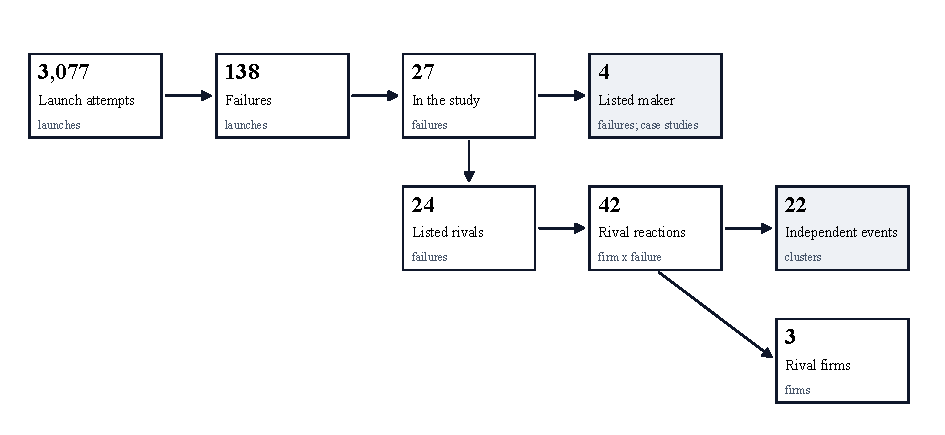
\includegraphics[width=\textwidth]{fig-sample.pdf}
\par\vspace{2pt}{\footnotesize Each box gives a count and its unit, and the unit changes along the way. Failures: GCAT success score below 0.75. In the study: the failure has a listed maker or a listed Tier 1-2 competitor (one failure has both). Competitor reactions: one per listed competitor per failure. Independent events: failures that share a firm within 5 trading days are grouped. Source: GCAT (McDowell, n.d.) and the project pipeline.}
\end{figure}

\subsection*{4.5 Event timing verification}
Day 0 depends on when a failure became public relative to the close of the exchange, so the disclosure time of each event was checked. For each event the time is either a sourced company statement, recorded with high or low confidence, or the launch time recorded in GCAT. GCAT times are used only where day 0 would not change if the true disclosure came 10 minutes earlier or up to 180 minutes later; events that fail this check need a sourced time. 88\% of competitor reactions (37 of 42) and 4 of 4 maker cases rely on GCAT launch times that were not checked separately against a company statement, and 2 competitor reactions rely on a sourced time with low confidence. Checks R5a and R5b (\hyperlink{s7}{section 7}) test whether these choices matter. \hyperlink{tab-tsrc}{Table 1} and \hyperlink{fig-timing}{Figure 2} give the breakdown.

\par\noindent\begin{minipage}{\textwidth}\hypertarget{tab-tsrc}{}
\textbf{Table 1.} Disclosure-time sources

{\small\setlength{\tabcolsep}{4pt}\begin{tabularx}{\textwidth}{Xlll}
\toprule
\textbf{Source of the disclosure time} & \textbf{Competitor reactions} & \textbf{Competitor failures} & \textbf{Maker cases} \\
\midrule
Company statement, high confidence & 3 & 2 & 0 \\
Company statement, low confidence & 2 & 1 & 0 \\
GCAT launch time (not separately verified) & 37 & 21 & 4 \\
\bottomrule
\end{tabularx}}
\vspace{6pt}

\end{minipage}\par\vspace{4pt}

\begin{figure}[htbp]\centering\hypertarget{fig-timing}{}
\caption*{\textbf{Figure 2.} Event timing verification}
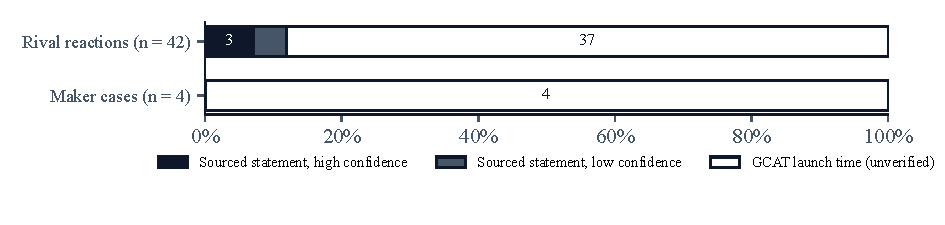
\includegraphics[width=\textwidth]{fig-timing.pdf}
\par\vspace{2pt}{\footnotesize Share of events by disclosure-time source. Competitor reactions: n = 42; maker cases: n = 4. Source: data/manual/disclosure\_times.csv and GCAT.}
\end{figure}

\subsection*{4.6 Description of the sample}
\hyperlink{fig-years}{Figure 3} shows how many orbital launch failures happened each year and how many of them enter the study. Most failures do not enter, because neither the maker nor any competitor was a listed launch firm at the time (\hyperlink{apx-e}{Appendix E}). \hyperlink{tab-desc}{Table 2} describes the competitor reactions firm by firm, and \hyperlink{fig-exposure}{Figure 4} shows which firm is present in each independent event. The cumulative abnormal return (CAR) in these tables is defined in \hyperlink{s5}{section 5}; in short, it is the part of a stock's move over the window that the market does not explain.

\begin{figure}[htbp]\centering\hypertarget{fig-years}{}
\caption*{\textbf{Figure 3.} Orbital launch failures per year}
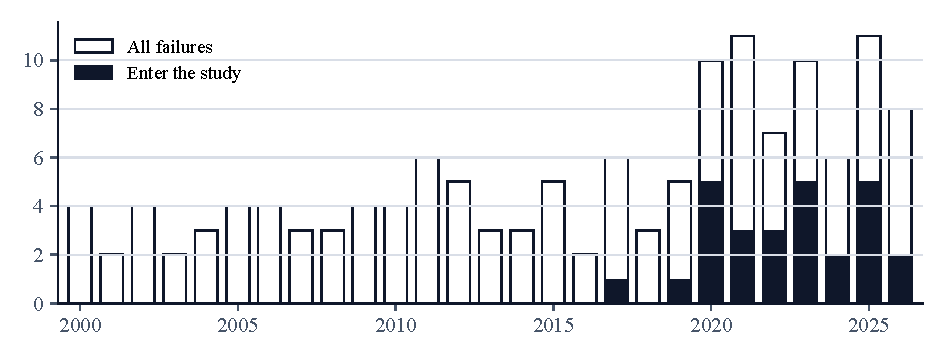
\includegraphics[width=\textwidth]{fig-years.pdf}
\par\vspace{2pt}{\footnotesize Outline: all orbital launch failures, 2000 to 2026. Filled: failures that enter the study.}
\end{figure}

\par\noindent\begin{minipage}{\textwidth}\hypertarget{tab-desc}{}
\textbf{Table 2.} Competitor reactions by firm, CAR T0 to T+1

{\small\setlength{\tabcolsep}{4pt}\begin{tabularx}{\textwidth}{Xllllll}
\toprule
\textbf{Firm} & \textbf{Ticker} & \textbf{Reactions} & \textbf{Clusters} & \textbf{Mean} & \textbf{Median} & \textbf{Range} \\
\midrule
Avio SpA & AVIO.MI & 24 & 22 & +0.60\% & +0.28\% & \textminus{}7.3\% to +14.5\% \\
Rocket Lab & RKLB & 15 & 14 & +0.79\% & +0.43\% & \textminus{}7.4\% to +25.3\% \\
Firefly Aerospace & FLY & 3 & 3 & \textminus{}4.86\% & \textminus{}6.07\% & \textminus{}7.0\% to \textminus{}1.5\% \\
\textbf{All} &  & 42 & 22 & +0.28\% & +0.28\% & \textminus{}7.4\% to +25.3\% \\
\bottomrule
\end{tabularx}}
\vspace{6pt}

Clusters: independent events in which the firm appears; 22 in total.

\end{minipage}\par\vspace{4pt}

\begin{figure}[htbp]\centering\hypertarget{fig-exposure}{}
\caption*{\textbf{Figure 4.} Which competitor is present in each independent event}
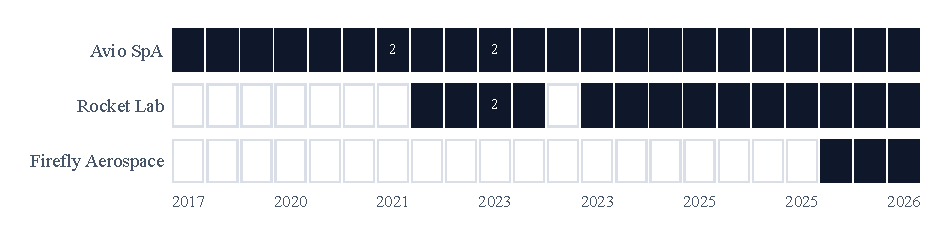
\includegraphics[width=\textwidth]{fig-exposure.pdf}
\par\vspace{2pt}{\footnotesize Columns: independent events in date order. Filled: the firm is a competitor in that event; a number means it appears more than once (two close failures).}
\end{figure}

\section*{\hypertarget{s5}{}5. Empirical methodology}
\subsection*{5.1 Normal and abnormal returns}
To measure the effect of a failure, the study first needs an estimate of how each stock would have moved without it. This "normal" return comes from the market model, which describes a stock's daily return as a constant plus a fixed share of the market's return (\hyperlink{ref-mackinlay1997}{MacKinlay, 1997}). The share is called beta (β): a stock with a beta of 1.5 tends to rise 1.5\% when the market rises 1\%. The model is estimated by ordinary least squares, the standard method that picks the line that best fits past data, on trading days 250 to 30 before day 0. This period, called the estimation window, ends a month before the event so that the event itself cannot affect the estimate. At least 100 daily returns are required. With 30 to 99 returns, the study uses a simpler market-adjusted model, in which the normal return is just the market return (α = 0 and β = 1), and flags the event:

\hypertarget{eq-1}{}\begin{equation}
R_{it} = \alpha_i + \beta_i R_{mt} + \varepsilon_{it}
\end{equation}

In \hyperlink{eq-1}{Equation 1}, \emph{R}\emph{it} is the return of stock \emph{i} on day \emph{t}, \emph{R}\emph{mt} is the return of its market index, and \emph{ε}\emph{it} is the part of the return that the market does not explain. The abnormal return (AR) on a day is the actual return minus the return the model predicts. The cumulative abnormal return (CAR) over an event window from day τ1 to day τ2 is the sum of the daily abnormal returns:

\hypertarget{eq-2}{}\begin{equation}
AR_{it} = R_{it} - (\hat\alpha_i + \hat\beta_i R_{mt}), \qquad CAR_i(\tau_1,\tau_2) = \sum_{t=\tau_1}^{\tau_2} AR_{it}
\end{equation}

A CAR of \textminus{}10\% over two days means that the stock did 10 percentage points worse than the market would have predicted, which can be read as the market cutting its estimate of the firm's value by about a tenth. Returns are simple percentage changes, and CARs are sums of simple abnormal returns.

\subsection*{5.2 How precise is each reaction?}
Each CAR contains noise, because even on a quiet day a stock does not move exactly as the model predicts. The variance of each CAR, a measure of how much it would vary by chance, includes both this daily noise and the error from estimating the model itself (\hyperlink{ref-campbell1997}{Campbell et al., 1997}). In \hyperlink{eq-3}{Equation 3}, \emph{σ̂}\emph{i}\textsuperscript{2} is the variance of the stock's unexplained returns in the estimation window, \emph{L} is the length of the event window, \emph{T} the number of estimation days, \emph{W} the event window and \emph{E} the estimation window:

\hypertarget{eq-3}{}\begin{equation}
\mathrm{Var}(CAR_i) = \hat\sigma_i^2\left[L + \frac{L^2}{T} + \frac{\left(\sum_{t\in W}(R_{mt}-\bar R_m)\right)^2}{\sum_{t\in E}(R_{mt}-\bar R_m)^2}\right]
\end{equation}

\subsection*{5.3 Testing whether competitors react}
A statistical test asks whether an average reaction is larger than chance alone would produce. Its result is summarized by a p-value: the probability of seeing an average at least this far from zero if the true average were zero. A p-value below 0.05 is the usual threshold for calling an effect statistically significant. The confirmatory test in this paper is the standardized test of \hyperlink{ref-boehmer1991}{Boehmer et al. (1991)}, called the BMP test. It first divides each CAR by its own standard deviation, so that every reaction is measured in units of its own noise, and then tests whether the average of these standardized CARs (SCARs) is zero. Because it uses the spread of the standardized CARs across firms, it remains valid when the failure makes returns more volatile than usual:

\hypertarget{eq-4}{}\begin{equation}
SCAR_i = \frac{CAR_i}{\sqrt{\mathrm{Var}(CAR_i)}}, \qquad t_{BMP} = \frac{\sqrt{N}\,\overline{SCAR}}{s_{SCAR}}
\end{equation}

One failure can hit several competitors on the same day, and their reactions are then not independent. The BMP statistic is therefore adjusted as proposed by \hyperlink{ref-kolari2010}{Kolari and Pynnönen (2010)} (the BMP-KP test, \hyperlink{eq-5}{Equation 5}). Correlation is allowed only within a cluster \emph{c}. For a pair of reactions it is the correlation of their unexplained returns in the estimation window, scaled by the share ℓ\emph{ij} of event-window days that the two windows have in common. The p-values use a t distribution with \emph{G} \textminus{} 1 degrees of freedom, where \emph{G} is the number of independent events; using the number of events rather than the number of reactions makes the test more cautious:

\hypertarget{eq-5}{}\begin{equation}
t_{KP} = t_{BMP}\sqrt{\frac{1-\bar r}{1+(N-1)\bar r}}, \quad \bar r = \frac{\sum_{i\neq j,\,c(i)=c(j)} \rho_{ij}}{N(N-1)}, \quad \rho_{ij} = \mathrm{corr}(\varepsilon_i,\varepsilon_j)\,\frac{\ell_{ij}}{L}
\end{equation}

The equal-weighted average CAR is reported with a cluster-robust interval (\hyperlink{eq-6}{Equation 6}). A cluster-robust standard error measures the uncertainty of the average while allowing reactions in the same independent event to be correlated. The 95\% interval is the range of values that the data cannot rule out at the 5\% level. As a further check, the study also reports a wild cluster bootstrap p-value, which re-creates the test many times from the data and is more reliable when there are few clusters (\hyperlink{ref-cameron2008}{Cameron et al., 2008}; \hyperlink{ref-webb2023}{Webb, 2023}):

\hypertarget{eq-6}{}\begin{equation}
SE_{CR} = \frac{1}{N}\sqrt{\frac{G}{G-1}\sum_g\Big(\sum_{i\in g}(CAR_i-\overline{CAR})\Big)^2}, \qquad \overline{CAR} \pm t_{G-1,\,0.975}\,SE_{CR}
\end{equation}

\subsection*{5.4 What exactly is being averaged?}
An average depends on how much weight each observation gets, and with few firms and events this choice matters. Let \emph{i} = 1, …, \emph{N} index competitor reactions (one per listed competitor per failure), \emph{g} = 1, …, \emph{G} independent events, and \emph{k} = 1, …, \emph{K} firms, with \emph{N}\emph{g} and \emph{N}\emph{k} reactions in event \emph{g} and firm \emph{k}, and \emph{s}\emph{i} = √Var(\emph{CAR}\emph{i}). Four averages answer four different questions. Statisticians call the quantity that an average is meant to measure the estimand:

\hypertarget{eq-7}{}\begin{equation}
\begin{gathered}\theta_{obs} = \frac{1}{N}\sum_i CAR_i,\qquad \theta_{event} = \frac{1}{G}\sum_g \frac{1}{N_g}\sum_{i\in g} CAR_i,\\ \theta_{prec} = \frac{\sum_i CAR_i/s_i}{\sum_i 1/s_i},\qquad \theta_{firm} = \frac{1}{K}\sum_k \frac{1}{N_k}\sum_{i\in k} CAR_i\end{gathered}
\end{equation}

\emph{θ}obs is the average reaction of a listed competitor to a failure; \emph{θ}event treats every independent event equally; \emph{θ}prec gives more weight to calm stocks, whose reactions are measured more precisely; and \emph{θ}firm treats every firm equally. The confirmatory hypothesis H2 is stated for \emph{θ}obs, reported with the cluster-robust interval of \hyperlink{eq-6}{Equation 6}. The prespecified BMP-KP test asks a slightly different question, whether the average standardized CAR is zero; the two coincide only when all stocks are about equally volatile, and the test is closest in spirit to \emph{θ}prec. Both are reported, each next to the quantity it matches. None of the weightings is better on statistical grounds; \emph{θ}obs stays the main estimate because it was chosen before the results were seen.

\subsection*{5.5 Event windows and prespecified checks}
The main window covers day 0 and the next trading day, which is long enough to capture a failure late in the trading day and short enough to keep out most other news. \hyperlink{tab-win}{Table 3} lists the windows. Nine robustness checks were fixed in advance. Check R1 averages the reactions within each independent event first and then tests the event averages, with both a t-test and a sign test, which counts how many averages are negative. Check R2 is a plain t-test that ignores standardization. Check R3 is a rank test in the spirit of \hyperlink{ref-corrado1989}{Corrado (1989)}, with a p-value obtained by simulation. Check R4 uses the wider window. Check R5 drops or shifts events whose disclosure time is uncertain. Check R6 drops reactions estimated with the market-adjusted fallback model. Check R7 drops clusters that contain more than one failure. Check R8 leaves out one firm at a time. Check R9 is a placebo test, which repeats the whole calculation on ordinary days with no failure, to see how often an average as large as the real one appears by chance. Analyses designed after the results were seen are called exploratory, are labelled wherever they appear, and never replace H2.

\par\noindent\begin{minipage}{\textwidth}\hypertarget{tab-win}{}
\textbf{Table 3.} Event windows

{\small\setlength{\tabcolsep}{4pt}\begin{tabularx}{\textwidth}{llX}
\toprule
\textbf{Window} & \textbf{Days} & \textbf{Role} \\
\midrule
Main & T0 to T+1 & Confirmatory test (H2) \\
Wider & T\textminus{}1 to T+3 & Robustness check \\
One month & T0 to T+20 & Description only \\
\bottomrule
\end{tabularx}}
\vspace{6pt}

\end{minipage}\par\vspace{4pt}

\section*{\hypertarget{s6}{}6. Main results}
\subsection*{6.1 The rocket's maker}
In every one of the 4 listed cases the maker's shares fell over the two trading days after the failure became public, after allowing for the movement of the market, by between \textminus{}8.8\% and \textminus{}16.3\%, and in each case the 95\% interval excludes zero. \hyperlink{tab-case}{Table 4} gives the numbers and \hyperlink{fig-paths}{Figure 5} shows how the losses built up over the days after each failure. In economic terms, investors cut their estimate of the maker's market value by 8.8\% to 16.3\% within two days. Losses of this size are consistent with investors expecting costs well beyond the lost rocket, such as delayed launches, lost contracts and a weaker reputation for reliability. With 4 cases from 2 firms, however, these are case studies, not an estimate of an average effect.

\par\noindent\begin{minipage}{\textwidth}\hypertarget{tab-case}{}
\textbf{Table 4.} The rocket's maker: two-day abnormal returns

{\small\setlength{\tabcolsep}{4pt}\begin{tabularx}{\textwidth}{llXlll}
\toprule
\textbf{Rocket} & \textbf{Failure} & \textbf{Listed maker} & \textbf{CAR T0 to T+1} & \textbf{95\% interval} & \textbf{CAR T\textminus{}1 to T+3} \\
\midrule
Vega & 11 Jul 2019 & Avio SpA (AVIO.MI) & \textminus{}12.3\% & \textminus{}15.9\% to \textminus{}8.7\% & \textminus{}11.0\% \\
Vega & 17 Nov 2020 & Avio SpA (AVIO.MI) & \textminus{}16.3\% & \textminus{}21.9\% to \textminus{}10.6\% & \textminus{}14.1\% \\
Vega C & 21 Dec 2022 & Avio SpA (AVIO.MI) & \textminus{}8.8\% & \textminus{}15.9\% to \textminus{}1.7\% & \textminus{}9.3\% \\
Electron & 19 Sep 2023 & Rocket Lab (RKLB) & \textminus{}10.5\% & \textminus{}19.6\% to \textminus{}1.4\% & \textminus{}7.2\% \\
\bottomrule
\end{tabularx}}
\vspace{6pt}

Intervals: CAR ± 1.96 × prediction-error standard deviation.

\end{minipage}\par\vspace{4pt}

\begin{figure}[htbp]\centering\hypertarget{fig-paths}{}
\caption*{\textbf{Figure 5.} The rocket's maker: cumulative abnormal return}
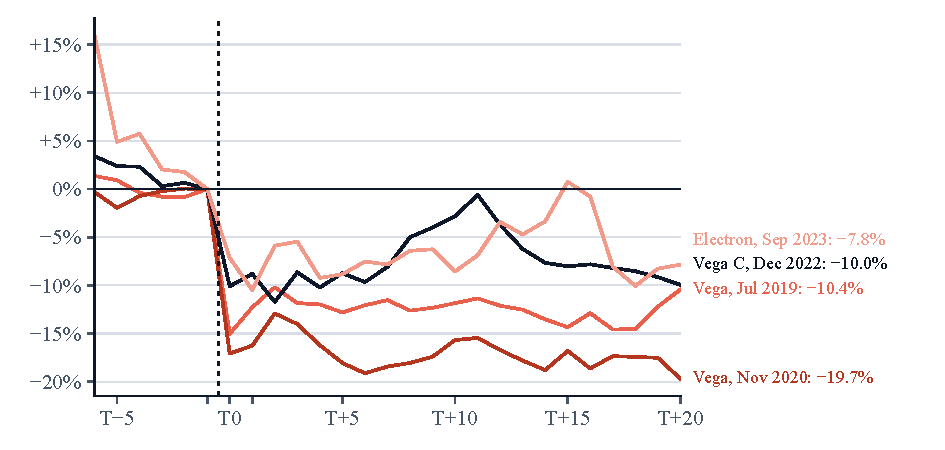
\includegraphics[width=\textwidth]{fig-paths.pdf}
\par\vspace{2pt}{\footnotesize Cumulative abnormal return from T\textminus{}5 to T+20, set to zero at the close before the failure (T\textminus{}1), so the value at T+1 is the two-day result in the table. 4 cases, market model, simple returns, home-market index. Source: project pipeline (prices from Yahoo Finance, not published).}
\end{figure}

\subsection*{6.2 Listed competitors}
\hyperlink{tab-inf}{Table 5} reports the confirmatory test. The equal-weighted average two-day abnormal return of listed competitors is +0.28\%, with a 95\% interval from \textminus{}1.62\% to +2.18\%; the cluster-robust p-value is 0.76 and the wild cluster bootstrap p-value is 0.85. The prespecified standardized test gives t = 0.85 (p = 0.40). H2 is therefore not rejected at the 5\% level by any of these tests.

In economic terms, the point estimate says that the average competitor's market value rose by about 0.28\% more than the market predicted over the two days after a failure. For a competitor worth one billion dollars, this would be a gain of about 2.8 million dollars. The interval, however, runs from \textminus{}1.62\% to +2.18\%, so a small loss through contagion and a small gain through competition are both consistent with the data.

\par\noindent\begin{minipage}{\textwidth}\hypertarget{tab-inf}{}
\textbf{Table 5.} Confirmatory test of H2: listed competitors, CAR T0 to T+1

{\small\setlength{\tabcolsep}{4pt}\begin{tabularx}{\textwidth}{Xl}
\toprule
\textbf{Quantity} & \textbf{Value} \\
\midrule
Mean CAR, equal weight per reaction & +0.28\% \\
95\% cluster-robust interval (t, G\textminus{}1 df) & \textminus{}1.62\% to +2.18\% \\
Mean standardized CAR (BMP) & 0.227 \\
BMP t, unadjusted & 0.932 \\
Kolari-Pynnönen adjustment factor & 0.916 \\
BMP-KP adjusted t / p (prespecified test; mean standardized CAR = 0) & 0.854 / 0.40 \\
Cluster-robust t / p for the mean CAR (matches the interval) & 0.306 / 0.76 \\
Wild cluster bootstrap p for the mean CAR (Webb weights, 9,999 draws) & 0.85 \\
Mean within-cluster correlation & 0.150 \\
Reactions / failures / firms / clusters & 42 / 24 / 3 / 22 \\
Minimum detectable effect (80\% / 90\% power) & 2.7\% / 3.1\% \\
Power against a true ±1\% / ±2\% / ±3\% mean & 0.18 / 0.55 / 0.88 \\
90\% interval (for an equivalence reading) & \textminus{}1.29\% to +1.85\% \\
\bottomrule
\end{tabularx}}
\vspace{6pt}

Minimum detectable effect: two-sided 5\% test, from the cluster-robust standard error implied by the interval.

\end{minipage}\par\vspace{4pt}

How large would an effect have to be for this sample to find it? With a cluster-robust standard error of 0.91\%, an average effect would need to be about 2.7\% to be detected four times out of five (80\% power), and about 3.1\% to be detected nine times out of ten. The chance of detecting a true average effect of 1\% is only 0.18. This figure is called the minimum detectable effect: the smallest true effect that a test of this size would usually find. A two-day move of 2.7\% in a firm's value is large in economic terms, so the test can only rule out large effects. The 90\% interval (\textminus{}1.29\% to +1.85\%) could support a claim that the effect is negligible only if a two-day effect of about ±1.9\% were accepted as negligible, which it is not. The data therefore do not show that competitors are unaffected; they show that any average effect is too small, relative to the noise, to be measured with this sample.

\subsection*{6.3 Sample concentration, repeated firm exposure, and external validity}
The competitor sample is concentrated. Avio SpA appears in every one of the 22 independent events. The same shares appear in many events, so the 22 clusters are not 22 independent draws from the launch industry. Grouping by event handles competitors that react on the same day, but a firm-specific shock that lasts for months, such as a change in how investors value one firm, links that firm's reactions across events. Grouping by firm would address this, but with 3 firms such inference is not reliable.

\par\noindent\begin{minipage}{\textwidth}\hypertarget{tab-contrib}{}
\textbf{Table 6.} Contribution of each firm to the competitor average

{\small\setlength{\tabcolsep}{4pt}\begin{tabularx}{\textwidth}{lllXl}
\toprule
\textbf{Firm} & \textbf{Reactions} & \textbf{Share of reactions} & \textbf{Contribution to the mean} & \textbf{Firm mean} \\
\midrule
Avio SpA & 24 & 57\% & +0.34\% & +0.60\% \\
Rocket Lab & 15 & 36\% & +0.28\% & +0.79\% \\
Firefly Aerospace & 3 & 7\% & \textminus{}0.35\% & \textminus{}4.86\% \\
\bottomrule
\end{tabularx}}
\vspace{6pt}

Contribution: the firm's summed CARs divided by all 42 reactions; contributions add up to the equal-weighted mean (+0.28\%).

\end{minipage}\par\vspace{4pt}

The average is close to zero partly because firms with opposite reactions cancel each other out. Firefly Aerospace's 3 reactions add \textminus{}0.35\% to the mean, while Avio SpA's 24 reactions add +0.34\% (\hyperlink{tab-contrib}{Table 6}). Weighting each firm equally instead of each reaction gives a different answer, and no weighting is better than the others on statistical grounds (\hyperlink{tab-wt}{Table 7} and \hyperlink{fig-weights}{Figure 6}). The every-reaction average is the main estimate only because it was chosen before the results were seen.

\par\noindent\begin{minipage}{\textwidth}\hypertarget{tab-wt}{}
\textbf{Table 7.} The competitor average under alternative weightings

{\small\setlength{\tabcolsep}{4pt}\begin{tabularx}{\textwidth}{XlX}
\toprule
\textbf{Weighting (estimand)} & \textbf{Estimate} & \textbf{Note} \\
\midrule
Every reaction equal (prespecified estimand) & +0.28\% & the main estimate \\
Every independent event equal & +0.21\% & same as the R1 portfolio average \\
Inverse prediction-error SD & +0.87\% & closest to the BMP statistic \\
Every firm equal & \textminus{}1.16\% & each firm's mean, then averaged \\
Median reaction & +0.28\% & not driven by a few large moves \\
\bottomrule
\end{tabularx}}
\vspace{6pt}

Sensitivity analysis added after the audit; the prespecified estimate is the first row.

\end{minipage}\par\vspace{4pt}

\begin{figure}[htbp]\centering\hypertarget{fig-weights}{}
\caption*{\textbf{Figure 6.} The competitor average under alternative weightings}
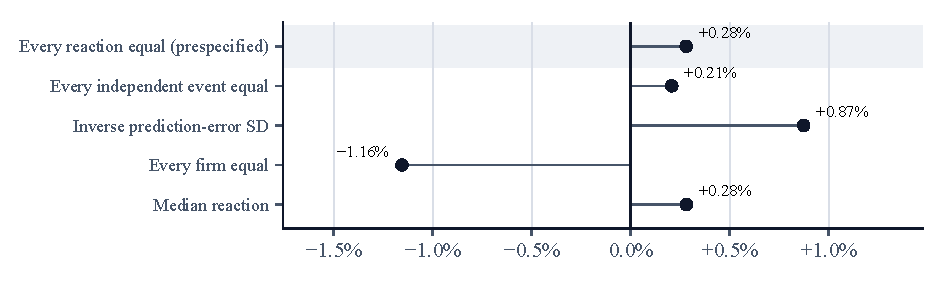
\includegraphics[width=\textwidth]{fig-weights.pdf}
\par\vspace{2pt}{\footnotesize CAR T0 to T+1, market model, simple returns; 42 reactions, 22 events, 3 firms. Shaded: the prespecified estimand.}
\end{figure}

A firm-level view makes the same point. The mean of the 3 firm means is \textminus{}1.16\%, with a 95\% interval of \textminus{}9.1\% to +6.8\%, but this interval rests on only 2 degrees of freedom and is therefore very wide. Leaving one firm out at a time (check R8, \hyperlink{s7}{section 7}) is the more informative check of how much the result depends on a single firm. The results describe these listed firms, not private, state-owned or diversified aerospace companies, and they cannot be extended to the launch industry as a whole.

\section*{\hypertarget{s7}{}7. Robustness and sensitivity}
A robustness check repeats the analysis with a different but reasonable choice, to see whether the conclusion depends on that choice. None of the 12 prespecified checks finds a significant average at the 5\% level (\hyperlink{fig-forest}{Figure 7} and \hyperlink{tab-rob}{Table 8}). The conclusion that no effect is detectable is therefore stable. The size of the estimate is not: across the checks the average ranges from \textminus{}0.15\% (Leave out AVIO.MI) to +1.84\% (Wider window, T\textminus{}1 to T+3). Leaving out one firm changes the sign of the average.

\begin{figure}[htbp]\centering\hypertarget{fig-forest}{}
\caption*{\textbf{Figure 7.} Listed competitors: main test and prespecified checks}
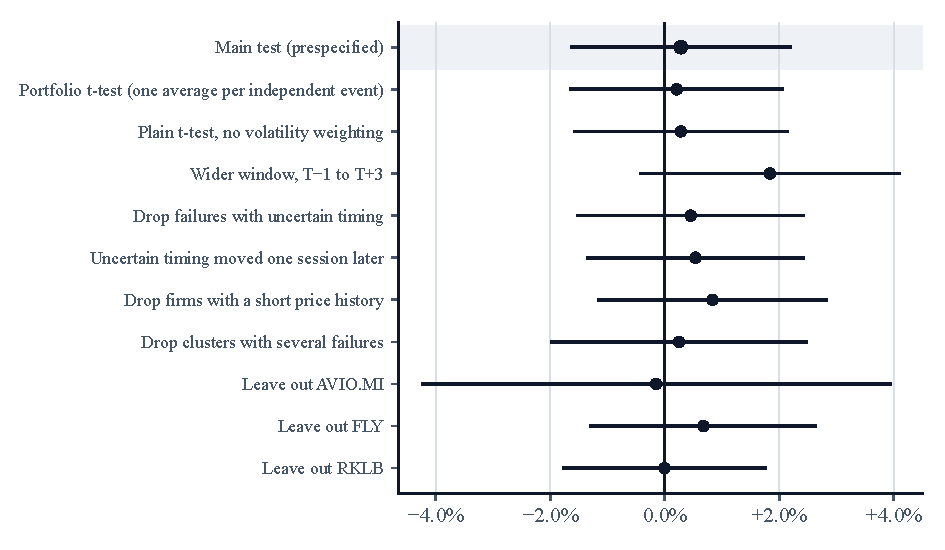
\includegraphics[width=\textwidth]{fig-forest.pdf}
\par\vspace{2pt}{\footnotesize Dots: average CAR T0 to T+1 (except the wider-window check); lines: 95\% cluster-robust intervals; tests without an interval are omitted. Full sample: 42 reactions, 22 events. Shaded: the confirmatory estimate.}
\end{figure}

\par\noindent\begin{minipage}{\textwidth}\hypertarget{tab-rob}{}
\textbf{Table 8.} Prespecified robustness checks

{\small\setlength{\tabcolsep}{4pt}\begin{tabularx}{\textwidth}{Xlllll}
\toprule
\textbf{Check} & \textbf{Average} & \textbf{95\% interval} & \textbf{p} & \textbf{Reactions} & \textbf{Clusters} \\
\midrule
Portfolio t-test (one average per independent event) & +0.21\% & \textminus{}1.63\% to +2.05\% & 0.82 & 42 & 22 \\
Sign test (share of events with a positive average) & +0.21\% & test only & 0.29 & 42 & 22 \\
Plain t-test, no volatility weighting & +0.28\% & \textminus{}1.57\% to +2.13\% & 0.76 & 42 & 22 \\
Rank test (simulated p-value) & +0.28\% & test only & 0.44 & 42 & 22 \\
Wider window, T\textminus{}1 to T+3 & +1.84\% & \textminus{}0.41\% to +4.09\% & 0.18 & 42 & 22 \\
Drop failures with uncertain timing & +0.45\% & \textminus{}1.52\% to +2.42\% & 0.37 & 40 & 21 \\
Uncertain timing moved one session later & +0.54\% & \textminus{}1.34\% to +2.41\% & 0.29 & 42 & 22 \\
Drop firms with a short price history & +0.83\% & \textminus{}1.15\% to +2.81\% & 0.27 & 38 & 21 \\
Drop clusters with several failures & +0.25\% & \textminus{}1.97\% to +2.47\% & 0.37 & 36 & 20 \\
Leave out AVIO.MI & \textminus{}0.15\% & \textminus{}4.23\% to +3.93\% & 0.77 & 18 & 14 \\
Leave out FLY & +0.68\% & \textminus{}1.28\% to +2.63\% & 0.30 & 39 & 22 \\
Leave out RKLB & 0.00\% & \textminus{}1.76\% to +1.75\% & 0.52 & 27 & 22 \\
\bottomrule
\end{tabularx}}
\vspace{6pt}

\end{minipage}\par\vspace{4pt}

The placebo test (R9) repeats the calculation on 1000 sets of randomly chosen ordinary trading days. If the real result were unusual, it would sit far in the tails of these placebo averages. It sits at the 61st percentile, with a two-sided share of 0.776, meaning that about 78\% of random sets give an average at least as far from zero (\hyperlink{fig-placebo}{Figure 8}). Because R9 draws a separate date for each reaction, it ignores that competitors hit by one failure move on the same day, so its spread is too narrow. It is a benchmark, not an exact test, and the percentile is not the probability that the effect is real. A version designed after the results, with one shared random date for all reactions in a cluster (R9b, 1000 draws), places the real result at the 66th percentile (two-sided share 0.684).

\begin{figure}[htbp]\centering\hypertarget{fig-placebo}{}
\caption*{\textbf{Figure 8.} Real result against random ordinary days (R9)}
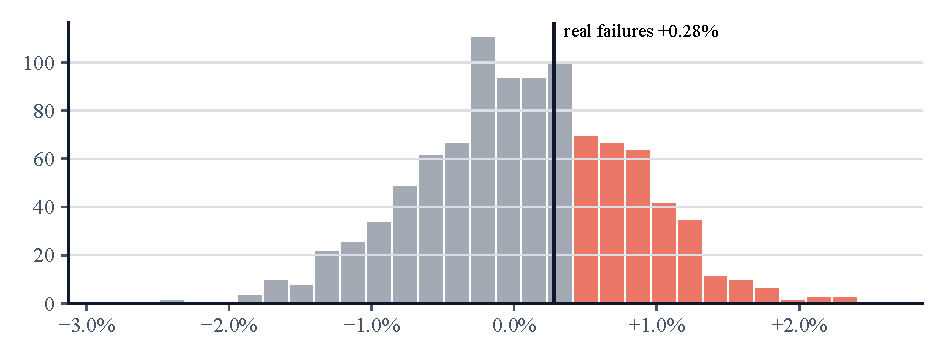
\includegraphics[width=\textwidth]{fig-placebo.pdf}
\par\vspace{2pt}{\footnotesize Average CAR T0 to T+1 over 42 reactions on random non-event days, 1000 draws (fixed seed), one random day per reaction. Red: averages at least as far out as the real result. Black line: the real failures. A benchmark, not an exact permutation test.}
\end{figure}

\section*{\hypertarget{s8}{}8. Confounding corporate announcements and sensitivity of the competitor estimate}
An event study gives the event credit for every unusual return in the window. If a firm announces something else on the same days, such as a new contract or quarterly results, its reaction mixes the two pieces of news. This problem is called confounding, and the event-study model cannot fix it by itself (\hyperlink{ref-mackinlay1997}{MacKinlay, 1997}). The news around the largest competitor reactions was therefore checked against public sources. \hyperlink{tab-flag}{Table 9} lists every competitor reaction with other company news in the window, the verdict, and the source of the news. Flagged reactions stay in the confirmatory test, because the rules fixed in advance do not allow events to be removed after the results are seen.

\par\noindent\begin{minipage}{\textwidth}\hypertarget{tab-flag}{}
\textbf{Table 9.} Competitor reactions with other news in the window

{\small\setlength{\tabcolsep}{4pt}\begin{tabularx}{\textwidth}{lXllX}
\toprule
\textbf{Firm} & \textbf{Failure} & \textbf{CAR} & \textbf{Verdict} & \textbf{News} \\
\midrule
Rocket Lab & Firefly Alpha, 22 Dec 2023 & +25.27\% & confounded & USD 515m Space Development Agency contract announced in the same window \href{https://www.fool.com/investing/2023/12/22/why-rocket-lab-stock-is-going-to-the-moon-today}{[source]} \\
Avio SpA & Kairos, 18 Dec 2024 & +14.51\% & confounded & EUR 350m ESA contracts released 18 Dec 2024 after the Milan close (day +1) \href{https://www.emarketstorage.it/sites/default/files/comunicati/2024-12/20241218_158732.pdf}{[source]} \\
Firefly Aerospace & PSLV-DL, 12 Jan 2026 & \textminus{}6.98\% & possibly confounded & Securities class-action lead-plaintiff deadline on day 0 \href{https://finviz.com/news/268191/shareholders-of-firefly-aerospace-inc-should-contact-levi-korsinsky-before-january-12-2026-to-discuss-your-rights-fly}{[source]} \\
Rocket Lab & Spectrum, 31 Mar 2025 & \textminus{}6.49\% & sector move & Broad tech and space-stock selloff on day 0 not absorbed by the S\&P 500 benchmark \href{https://finviz.com/news/13588/why-rocket-lab-planet-labs-and-ast-spacemobile-stocks-all-dropped-on-monday}{[source]} \\
\bottomrule
\end{tabularx}}
\vspace{6pt}

\end{minipage}\par\vspace{4pt}

The exploratory specifications in \hyperlink{tab-conf}{Table 10} and \hyperlink{fig-conf}{Figure 9} drop the flagged reactions. Dropping the 2 reactions that coincide with contract news changes the average from +0.28\% to \textminus{}0.70\%, but the median moves only from +0.28\% to +0.09\%. The change therefore comes from removing two large positive moves, not from a shift in the typical reaction. The standardized test hardly moves (p = 0.86), because it already gives less weight to the volatile stocks behind those moves. These exploratory estimates are not more correct than the prespecified one, because the choice of what to drop was made after seeing the data.

\par\noindent\begin{minipage}{\textwidth}\hypertarget{tab-conf}{}
\textbf{Table 10.} Confounding-news sensitivity (exploratory)

{\small\setlength{\tabcolsep}{4pt}\begin{tabularx}{\textwidth}{Xllllll}
\toprule
\textbf{Specification} & \textbf{Average} & \textbf{95\% interval} & \textbf{p} & \textbf{Median} & \textbf{Reactions} & \textbf{Clusters} \\
\midrule
Main test (prespecified) & +0.28\% & \textminus{}1.62\% to +2.18\% & 0.40 & +0.28\% & 42 & 22 \\
Drop the contract-news days (exploratory) & \textminus{}0.70\% & \textminus{}1.80\% to +0.39\% & 0.86 & +0.09\% & 40 & 22 \\
Also drop possible same-day news (exploratory) & \textminus{}0.54\% & \textminus{}1.71\% to +0.63\% & 0.95 & +0.26\% & 39 & 22 \\
Drop every flagged day (exploratory) & \textminus{}0.38\% & \textminus{}1.58\% to +0.82\% & 0.95 & +0.28\% & 38 & 22 \\
\bottomrule
\end{tabularx}}
\vspace{6pt}

\end{minipage}\par\vspace{4pt}

\begin{figure}[htbp]\centering\hypertarget{fig-conf}{}
\caption*{\textbf{Figure 9.} Confounding-news sensitivity}
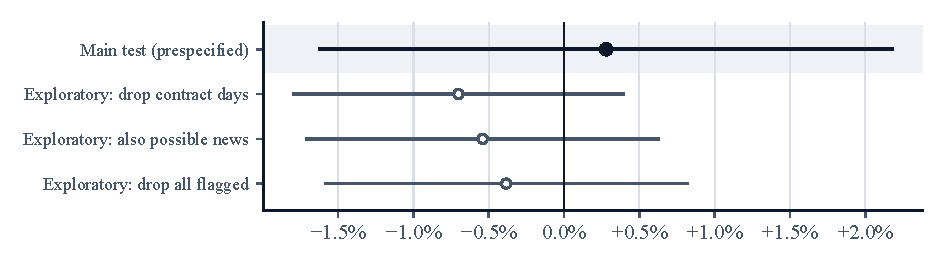
\includegraphics[width=\textwidth]{fig-conf.pdf}
\par\vspace{2pt}{\footnotesize Average CAR T0 to T+1 with 95\% cluster-robust intervals. Shaded: the prespecified estimate (42 reactions). Hollow: exploratory specifications, chosen after results, that drop reactions with other news.}
\end{figure}

\section*{\hypertarget{s9}{}9. Discussion}
The evidence supports two statements. First, listed makers lose a large share of their value when their rocket fails, in a small set of cases. Second, the average reaction of listed competitors cannot be told apart from zero in this sample. The first finding fits the Challenger evidence, where the market quickly singled out the firm responsible for the failure (\hyperlink{ref-maloney2003}{Maloney \& Mulherin, 2003}). The second differs from the clear average contagion that \hyperlink{ref-lang1992}{Lang and Stulz (1992)} find for bankruptcies, although their finding that competitors can gain in concentrated industries shows that the net effect depends on the industry.

Several explanations are consistent with a small net reaction of competitors, and the data cannot separate them. Contagion and competitive gains may both be present and cancel each other out, as the two channels in \hyperlink{s1}{section 1} suggest. Customers may be unable to switch providers quickly, because rockets and satellites need long preparation and the choice of providers is limited (\hyperlink{ref-dillow2015}{Dillow, 2015}), which would weaken the competitive effect in the short run. Or investors may treat a failure mainly as news about the failed firm and its rocket rather than about the industry. A short-lived market-wide mood effect of the kind found after air crashes (\hyperlink{ref-kaplanski2010}{Kaplanski \& Levy, 2010}) would be removed by the market model, because it moves the benchmark index as well. Separating these explanations would need customer-level data on contracts that moved between providers, launch backlogs, or a much larger sample of listed competitors.

For investors, the results suggest that, in this sample, a launch failure is mainly a risk for the firm whose rocket failed rather than for the listed industry as a whole. The evidence is too weak, however, to treat competitors' shares as unaffected, and the conclusion may change as more launch firms list and the number of independent events grows.

\section*{\hypertarget{s10}{}10. Limitations}
The first limitation is the small number of listed firms. Only 3 listed firms qualify as competitors, and they produce 22 independent events, every one of which involves Avio SpA. Because the same shares appear in many events, grouping reactions by event captures only part of the dependence between them, and with 3 firms grouping by firm is not reliable either. The maker evidence is thinner still: 4 cases from 2 firms, which are case studies rather than an average effect.

The second limitation is statistical power. Average effects of about 2.7\% could go undetected, so the study cannot claim that the effect is zero or negligible. The sign of the estimate depends on how events and firms are weighted, and on two large reactions that coincide with contract news. The interval (for the equal-weighted mean) and the prespecified test (for the standardized mean) answer slightly different questions and can disagree.

The third limitation is timing. 88\% of competitor reactions and 4 of 4 maker cases use GCAT launch times that were not checked separately against a company statement. These times are used only where day 0 would not change if the true disclosure came up to 10 minutes earlier or 180 minutes later. One failure is dated by a statement with low confidence, which checks R5a and R5b address. A clock or time-zone error larger than that band would move day 0.

The fourth limitation is the model. A one-factor market model with a home-market index does not remove moves that affect the whole space sector on the event days (one flagged case). Firms that were listed but later delisted, such as Orbital Sciences (later Orbital ATK), Astra and Virgin Orbit, are missing from the main sample because the free price source does not carry them. Yahoo Finance prices and GCAT records are good sources but are not audited.

Finally, the results describe historically eligible, publicly traded launch firms with comparable commercial business, not the launch industry as a whole, and they say nothing about private, state-owned or diversified aerospace companies. The rules were committed to git before the results (\hyperlink{apx-g}{Appendix G}) but were not filed with an independent registry, and git timestamps are set by the author.

\section*{\hypertarget{s11}{}11. Conclusion}
When an orbital rocket fails, its listed maker loses a large share of its value within two days in every case observed. For listed competitors, the average two-day reaction is +0.28\%, with an interval from \textminus{}1.62\% to +2.18\%. The data do not establish contagion or competitive gains, and they do not rule out either at magnitudes of a few percent.

The study is useful as a transparent and reproducible starting point. Every number can be recomputed from the published data (\hyperlink{apx-d}{Appendix D}), and the rules were fixed before the results (\hyperlink{apx-g}{Appendix G}). Adding more listed firms, including firms that have since delisted, and adding SpaceX as its price history grows, would sharpen the answer without changing the prespecified test.

\clearpage
\section*{\hypertarget{refs}{}References}
{\raggedright\setlength{\parskip}{8pt}
\noindent\hypertarget{ref-abramov2015}{}\hangindent=0.5in\hangafter=1 Abramov, D., \& Kiang, C. (2015). \emph{Effect of space launch delays and failures on stock market returns of commercial payload operators} (Paper IAC-15,E6,1,1,x29453) [Conference paper]. 66th International Astronautical Congress, Jerusalem, Israel. \url{https://iafastro.directory/iac/archive/browse/IAC-15/E6/1/29453/}\par
\noindent\hypertarget{ref-aharony1983}{}\hangindent=0.5in\hangafter=1 Aharony, J., \& Swary, I. (1983). Contagion effects of bank failures: Evidence from capital markets. \emph{Journal of Business, 56}(3), 305--322. \url{https://doi.org/10.1086/296203}\par
\noindent\hypertarget{ref-blose1996}{}\hangindent=0.5in\hangafter=1 Blose, L. E., Bornkamp, R., Brier, M., Brown, K., \& Frederick, J. (1996). Catastrophic events, contagion, and stock market efficiency: The case of the space shuttle Challenger. \emph{Review of Financial Economics, 5}(2), 117--129. \url{https://doi.org/10.1016/S1058-3300(96)90010-5}\par
\noindent\hypertarget{ref-boehmer1991}{}\hangindent=0.5in\hangafter=1 Boehmer, E., Musumeci, J., \& Poulsen, A. B. (1991). Event-study methodology under conditions of event-induced variance. \emph{Journal of Financial Economics, 30}(2), 253--272. \url{https://doi.org/10.1016/0304-405X(91)90032-F}\par
\noindent\hypertarget{ref-bosch1998}{}\hangindent=0.5in\hangafter=1 Bosch, J.-C., Eckard, E. W., \& Singal, V. (1998). The competitive impact of air crashes: Stock market evidence. \emph{Journal of Law and Economics, 41}(2), 503--519. \url{https://doi.org/10.1086/467399}\par
\noindent\hypertarget{ref-brown1985}{}\hangindent=0.5in\hangafter=1 Brown, S. J., \& Warner, J. B. (1985). Using daily stock returns: The case of event studies. \emph{Journal of Financial Economics, 14}(1), 3--31. \url{https://doi.org/10.1016/0304-405X(85)90042-X}\par
\noindent\hypertarget{ref-cameron2008}{}\hangindent=0.5in\hangafter=1 Cameron, A. C., Gelbach, J. B., \& Miller, D. L. (2008). Bootstrap-based improvements for inference with clustered errors. \emph{Review of Economics and Statistics, 90}(3), 414--427. \url{https://doi.org/10.1162/rest.90.3.414}\par
\noindent\hypertarget{ref-campbell1997}{}\hangindent=0.5in\hangafter=1 Campbell, J. Y., Lo, A. W., \& MacKinlay, A. C. (1997). \emph{The econometrics of financial markets}. Princeton University Press.\par
\noindent\hypertarget{ref-chance1987}{}\hangindent=0.5in\hangafter=1 Chance, D. M., \& Ferris, S. P. (1987). The effect of aviation disasters on the air transport industry: A financial market perspective. \emph{Journal of Transport Economics and Policy, 21}(2), 151--165. \url{https://doi.org/10.3828/jtep.1987.21.2.151}\par
\noindent\hypertarget{ref-corrado1989}{}\hangindent=0.5in\hangafter=1 Corrado, C. J. (1989). A nonparametric test for abnormal security-price performance in event studies. \emph{Journal of Financial Economics, 23}(2), 385--395. \url{https://doi.org/10.1016/0304-405X(89)90064-0}\par
\noindent\hypertarget{ref-cross2018}{}\hangindent=0.5in\hangafter=1 Cross, B., \& Vesely, W. (2018, September 16--21). \emph{Synthesizing a new launch vehicle failure probability based on historical flight data} [Conference presentation]. Probabilistic Safety Assessment and Management Conference (PSAM 14), Los Angeles, CA, United States. \url{https://ntrs.nasa.gov/citations/20180006947}\par
\noindent\hypertarget{ref-dillow2015}{}\hangindent=0.5in\hangafter=1 Dillow, C. (2015, July 23). What SpaceX’s launch failure means for the private space industry. \emph{Fortune}. \url{https://fortune.com/2015/07/23/spacex-rocket-failure-industry/}\par
\noindent\hypertarget{ref-do2023}{}\hangindent=0.5in\hangafter=1 Do, H. X., Nguyen, N. H., Nguyen, Q. M. P., \& Truong, C. (2023). Aerospace competition, investor attention, and stock return comovement. \emph{Journal of Economic Behavior \& Organization, 215}, 40--59. \url{https://doi.org/10.1016/j.jebo.2023.09.005}\par
\noindent\hypertarget{ref-fama1969}{}\hangindent=0.5in\hangafter=1 Fama, E. F., Fisher, L., Jensen, M. C., \& Roll, R. (1969). The adjustment of stock prices to new information. \emph{International Economic Review, 10}(1), 1--21. \url{https://doi.org/10.2307/2525569}\par
\noindent\hypertarget{ref-faa2021}{}\hangindent=0.5in\hangafter=1 Federal Aviation Administration. (2021). \emph{Part 450 mishap plan: Reporting, response, and investigation requirements} (Advisory Circular 450.173-1). U.S. Department of Transportation. \url{https://www.faa.gov/documentLibrary/media/Advisory_Circular/AC_450.173-1.pdf}\par
\noindent\hypertarget{ref-jarrell1985}{}\hangindent=0.5in\hangafter=1 Jarrell, G., \& Peltzman, S. (1985). The impact of product recalls on the wealth of sellers. \emph{Journal of Political Economy, 93}(3), 512--536. \url{https://doi.org/10.1086/261313}\par
\noindent\hypertarget{ref-kaplanski2010}{}\hangindent=0.5in\hangafter=1 Kaplanski, G., \& Levy, H. (2010). Sentiment and stock prices: The case of aviation disasters. \emph{Journal of Financial Economics, 95}(2), 174--201. \url{https://doi.org/10.1016/j.jfineco.2009.10.002}\par
\noindent\hypertarget{ref-kolari2010}{}\hangindent=0.5in\hangafter=1 Kolari, J. W., \& Pynnönen, S. (2010). Event study testing with cross-sectional correlation of abnormal returns. \emph{Review of Financial Studies, 23}(11), 3996--4025. \url{https://doi.org/10.1093/rfs/hhq072}\par
\noindent\hypertarget{ref-lang1992}{}\hangindent=0.5in\hangafter=1 Lang, L. H. P., \& Stulz, R. M. (1992). Contagion and competitive intra-industry effects of bankruptcy announcements. \emph{Journal of Financial Economics, 32}(1), 45--60. \url{https://doi.org/10.1016/0304-405X(92)90024-R}\par
\noindent\hypertarget{ref-mackinlay1997}{}\hangindent=0.5in\hangafter=1 MacKinlay, A. C. (1997). Event studies in economics and finance. \emph{Journal of Economic Literature, 35}(1), 13--39.\par
\noindent\hypertarget{ref-maloney2003}{}\hangindent=0.5in\hangafter=1 Maloney, M. T., \& Mulherin, J. H. (2003). The complexity of price discovery in an efficient market: The stock market reaction to the Challenger crash. \emph{Journal of Corporate Finance, 9}(4), 453--479. \url{https://doi.org/10.1016/S0929-1199(02)00055-X}\par
\noindent\hypertarget{ref-mcdowell}{}\hangindent=0.5in\hangafter=1 McDowell, J. C. (n.d.). \emph{GCAT: General catalog of artificial space objects} [Data set]. \url{https://planet4589.org/space/gcat/}\par
\noindent\hypertarget{ref-euronews2026}{}\hangindent=0.5in\hangafter=1 SpaceX makes its Nasdaq debut after the largest public offering in history. (2026, June 12). \emph{Euronews}. \url{https://www.euronews.com/business/2026/06/12/spacex-makes-its-nasdaq-debut-after-the-largest-public-offering-in-history}\par
\noindent\hypertarget{ref-webb2023}{}\hangindent=0.5in\hangafter=1 Webb, M. D. (2023). Reworking wild bootstrap-based inference for clustered errors. \emph{Canadian Journal of Economics, 56}(3), 839--858. \url{https://doi.org/10.1111/caje.12661}\par
\noindent\hypertarget{ref-yahoo}{}\hangindent=0.5in\hangafter=1 Yahoo Finance. (n.d.). \emph{Historical prices} [Data set]. \url{https://finance.yahoo.com/}\par
}

\clearpage
\hypertarget{apx}{}\section*{\hypertarget{apx-a}{}Appendix A. Competitor event list}
\hyperlink{tab-events}{Table 11} lists every competitor reaction in the confirmatory test, in date order, with the model used, the source of the disclosure time, any news flag, the two-day CAR and its standard deviation.

\hypertarget{tab-events}{}\textbf{Table 11.} All competitor reactions, CAR T0 to T+1

{\scriptsize\setlength{\tabcolsep}{4pt}\begin{xltabular}{\textwidth}{lllllllXll}
\toprule
\textbf{Failure} & \textbf{Rocket} & \textbf{T0} & \textbf{Ticker} & \textbf{Cluster} & \textbf{Model} & \textbf{Timing} & \textbf{Flag} & \textbf{CAR} & \textbf{SD} \\
\midrule
\endhead
2017-051 & PSLV-XL & 2017-08-31 & AVIO.MI & 58 & MA & high &  & \textminus{}0.86\% & 2.21\% \\
2020-F04 & LauncherOne & 2020-05-26 & AVIO.MI & 74 & MM & provisional &  & \textminus{}3.08\% & 2.73\% \\
2020-F05 & Electron & 2020-07-06 & AVIO.MI & 75 & MM & provisional &  & \textminus{}0.09\% & 2.88\% \\
2020-F07 & Astra Rocket 3.1 & 2020-09-14 & AVIO.MI & 76 & MM & provisional &  & \textminus{}4.32\% & 2.68\% \\
2020-F09 & Astra Rocket 3.2 & 2020-12-16 & AVIO.MI & 77 & MM & provisional &  & +2.99\% & 2.87\% \\
2021-F02 & Electron & 2021-05-17 & AVIO.MI & 81 & MM & provisional &  & +1.30\% & 3.02\% \\
2021-F07 & Astra Rocket 3.3 & 2021-08-30 & AVIO.MI & 84 & MM & provisional &  & +1.59\% & 3.26\% \\
2021-F08 & Firefly Alpha & 2021-09-03 & AVIO.MI & 84 & MM & provisional &  & \textminus{}3.77\% & 3.25\% \\
2022-F01 & Astra Rocket 3.3 & 2022-02-10 & RKLB & 87 & MA & high &  & \textminus{}6.00\% & 9.37\% \\
2022-F01 & Astra Rocket 3.3 & 2022-02-11 & AVIO.MI & 87 & MM & high &  & +0.26\% & 2.44\% \\
2022-F03 & Astra Rocket 3.3 & 2022-06-13 & AVIO.MI & 89 & MM & provisional &  & \textminus{}7.25\% & 2.82\% \\
2022-F03 & Astra Rocket 3.3 & 2022-06-13 & RKLB & 89 & MM & provisional &  & +0.43\% & 7.91\% \\
2023-F01 & LauncherOne & 2023-01-10 & AVIO.MI & 94 & MM & provisional &  & \textminus{}3.93\% & 3.64\% \\
2023-F01 & LauncherOne & 2023-01-10 & RKLB & 94 & MM & provisional &  & +3.31\% & 5.48\% \\
2023-F02 & RS1 & 2023-01-11 & AVIO.MI & 94 & MM & provisional &  & \textminus{}1.78\% & 3.65\% \\
2023-F02 & RS1 & 2023-01-11 & RKLB & 94 & MM & provisional &  & +7.33\% & 5.48\% \\
2023-F04 & Terran 1 & 2023-03-23 & AVIO.MI & 95 & MM & provisional &  & \textminus{}0.93\% & 3.42\% \\
2023-F04 & Terran 1 & 2023-03-23 & RKLB & 95 & MM & provisional &  & +0.72\% & 5.26\% \\
2023-F08 & Electron & 2023-09-19 & AVIO.MI & 98 & MM & provisional &  & \textminus{}0.56\% & 2.38\% \\
2023-202 & Firefly Alpha & 2023-12-22 & RKLB & 93 & MM & provisional & confounded & +25.27\% & 4.67\% \\
2023-202 & Firefly Alpha & 2023-12-27 & AVIO.MI & 93 & MM & provisional &  & +6.35\% & 1.84\% \\
2024-F01 & Kairos & 2024-03-13 & AVIO.MI & 100 & MM & provisional &  & +4.65\% & 1.75\% \\
2024-F01 & Kairos & 2024-03-13 & RKLB & 100 & MM & provisional &  & \textminus{}2.78\% & 5.05\% \\
2024-F04 & Kairos & 2024-12-18 & AVIO.MI & 103 & MM & provisional & confounded & +14.51\% & 2.65\% \\
2024-F04 & Kairos & 2024-12-18 & RKLB & 103 & MM & provisional &  & \textminus{}7.31\% & 5.99\% \\
2025-F04 & Spectrum & 2025-03-31 & AVIO.MI & 106 & MM & provisional &  & +2.69\% & 2.81\% \\
2025-F04 & Spectrum & 2025-03-31 & RKLB & 106 & MM & provisional & sector move & \textminus{}6.49\% & 6.99\% \\
2025-U01 & Firefly Alpha & 2025-04-29 & AVIO.MI & 111 & MM & low &  & +1.12\% & 3.00\% \\
2025-U01 & Firefly Alpha & 2025-04-29 & RKLB & 111 & MM & low &  & \textminus{}7.45\% & 7.15\% \\
2025-F05 & PSLV-XL & 2025-05-19 & AVIO.MI & 107 & MM & provisional &  & +3.37\% & 3.10\% \\
2025-F05 & PSLV-XL & 2025-05-19 & RKLB & 107 & MM & provisional &  & +0.85\% & 7.15\% \\
2025-F06 & Eris Block 1 & 2025-07-30 & AVIO.MI & 108 & MM & provisional &  & +0.41\% & 3.60\% \\
2025-F06 & Eris Block 1 & 2025-07-30 & RKLB & 108 & MM & provisional &  & +4.54\% & 7.40\% \\
2025-F09 & HANBIT-NANO & 2025-12-23 & AVIO.MI & 113 & MM & provisional &  & \textminus{}1.50\% & 5.50\% \\
2025-F09 & HANBIT-NANO & 2025-12-23 & FLY & 113 & MA & provisional &  & \textminus{}6.07\% & 7.54\% \\
2025-F09 & HANBIT-NANO & 2025-12-23 & RKLB & 113 & MM & provisional &  & \textminus{}2.83\% & 6.83\% \\
2026-F01 & PSLV-DL & 2026-01-12 & AVIO.MI & 115 & MM & provisional &  & +3.00\% & 5.58\% \\
2026-F01 & PSLV-DL & 2026-01-12 & FLY & 115 & MA & provisional & possibly confounded & \textminus{}6.98\% & 8.26\% \\
2026-F01 & PSLV-DL & 2026-01-12 & RKLB & 115 & MM & provisional &  & +1.83\% & 6.75\% \\
2026-F04 & Kairos & 2026-03-05 & AVIO.MI & 116 & MM & provisional &  & +0.30\% & 5.71\% \\
2026-F04 & Kairos & 2026-03-05 & FLY & 116 & MM & provisional &  & \textminus{}1.53\% & 9.37\% \\
2026-F04 & Kairos & 2026-03-05 & RKLB & 116 & MM & provisional &  & +0.43\% & 6.51\% \\
\bottomrule
\end{xltabular}}
\vspace{6pt}

Model: MM market model, MA market-adjusted fallback. SD: prediction-error standard deviation of the CAR.

\section*{\hypertarget{apx-b}{}Appendix B. Firm mapping and competitor criteria}
Competitors are classified point in time from two hand-built files. The firm map (\texttt{data/\allowbreak{}manual/\allowbreak{}firm\_\allowbreak{}map.csv}) records, for each firm and period, the listing dates, the ownership of each rocket, how important launch is to the firm, and the source of each fact. The size-and-market table (\texttt{data/\allowbreak{}manual/\allowbreak{}vehicle\_\allowbreak{}segments.csv}) records the size class and customer market of each rocket. A Tier 1 competitor must be listed, have launch as a pure-play or major business, sell a rocket of the same size class to the same customer market as the failed rocket, and have flown that rocket in the previous 730 days. Tier 2 competitors are added case by case in \texttt{data/\allowbreak{}manual/\allowbreak{}rival\_\allowbreak{}overrides.csv}, each with a source. Diversified aerospace groups are classified as having minor exposure to launch and enter only descriptive tiers, not the test.

\section*{\hypertarget{apx-c}{}Appendix C. Additional exploratory results}
\hyperlink{tab-expl}{Table 12} reports comparisons designed after the results were seen. Their p-values are adjusted with the Holm method, which raises each p-value to allow for the fact that several comparisons were made at once.

\par\noindent\begin{minipage}{\textwidth}\hypertarget{tab-expl}{}
\textbf{Table 12.} Exploratory comparisons (Holm-adjusted p-values)

{\small\setlength{\tabcolsep}{4pt}\begin{tabularx}{\textwidth}{Xlll}
\toprule
\textbf{Comparison} & \textbf{Estimate} & \textbf{p} & \textbf{p (Holm)} \\
\midrule
Competitors: first-flight failures minus other failures & \textminus{}1.33\% & 0.45 & 0.89 \\
Maker: failures minus successful launches & \textminus{}11.84\% & 0.002 & 0.005 \\
Competitors over one month (T0 to T+20) & +0.83\% & 0.72 & 0.89 \\
\bottomrule
\end{tabularx}}
\vspace{6pt}

\end{minipage}\par\vspace{4pt}

\section*{\hypertarget{apx-d}{}Appendix D. Statistical verification}
An independent script (\texttt{audit/\allowbreak{}verify\_\allowbreak{}published.py}) recomputes the published statistics from the published derived data, without importing any of the project's own code. 81 of 81 quantities match within a tolerance of 1e-9 for estimates and intervals and 1e-8 for test statistics and p-values. The CARs themselves need licensed prices and are reproduced by running the pipeline again.

\section*{\hypertarget{apx-e}{}Appendix E. Exclusions}
Most failures do not enter the study because neither the maker nor any competitor was a listed launch firm at the time. The reasons are counted below.

\par\noindent\begin{minipage}{\textwidth}\hypertarget{tab-why}{}
\textbf{Table 13.} Failures not in the study, by reason

{\small\setlength{\tabcolsep}{4pt}\begin{tabularx}{\textwidth}{Xl}
\toprule
\textbf{Reason} & \textbf{Failures} \\
\midrule
maker not a listed company & 97 \\
no listed maker or listed competitor & 13 \\
maker not listed, or not the owner, on that date & 1 \\
\bottomrule
\end{tabularx}}
\vspace{6pt}

A failure can have more than one reason, so the counts can add up to more than the number of excluded failures.

\end{minipage}\par\vspace{4pt}

\section*{\hypertarget{apx-f}{}Appendix F. Reproduction guide}
The full analysis can be reproduced with Python 3.11 or later. After installing the required packages with \texttt{pip install -r requirements.txt}, the script \texttt{pipeline/\allowbreak{}01\_\allowbreak{}ingest\_\allowbreak{}launches.py} downloads GCAT and classifies the launches, and \texttt{02\_\allowbreak{}map\_\allowbreak{}firms.py} applies the firm map. The script \texttt{03\_\allowbreak{}pull\_\allowbreak{}prices.py} downloads prices from Yahoo Finance, which are not redistributed, and \texttt{04\_\allowbreak{}check\_\allowbreak{}coverage.py} writes the feasibility check. The script \texttt{05\_\allowbreak{}event\_\allowbreak{}study.py} runs the prespecified analysis, and \texttt{06} and \texttt{09} run the exploratory checks. Finally, \texttt{07\_\allowbreak{}export\_\allowbreak{}site\_\allowbreak{}data.py} exports the derived statistics, \texttt{08\_\allowbreak{}build\_\allowbreak{}html.py} builds the website and this paper, \texttt{python audit/\allowbreak{}verify\_\allowbreak{}published.py} checks every published statistic again, and \texttt{python -m pytest tests} runs the test suite.

\section*{\hypertarget{apx-g}{}Appendix G. Freeze record}
The rules of the study (hypothesis, test, windows, sample criteria and checks) were committed to the public repository before the first results were computed. \hyperlink{tab-freeze}{Table 14} lists the commits. The published statistics were exported from commit \texttt{03b08fc} (with uncommitted changes in the working tree). Exploratory analyses added later (E1 to E3, R9b and the audit diagnostics) are labelled wherever they appear.

\par\noindent\begin{minipage}{\textwidth}\hypertarget{tab-freeze}{}
\textbf{Table 14.} Commit record

{\small\setlength{\tabcolsep}{4pt}\begin{tabularx}{\textwidth}{Xll}
\toprule
\textbf{Item} & \textbf{Commit} & \textbf{Time (+06:00)} \\
\midrule
Rules fixed (end of Phase 1) & \texttt{6e43dee} & 21 Nov 2026 20:13:38 \\
Phase 2 code; rules frozen before results & \texttt{54393b2} & 21 Nov 2026 20:30:24 \\
First results (step 05) & \texttt{be71a52} & 21 Nov 2026 20:31:18 \\
\bottomrule
\end{tabularx}}
\vspace{6pt}

\end{minipage}\par\vspace{4pt}

\section*{Where to find the charts, data and code}
{\small\setlength{\tabcolsep}{4pt}\begin{tabularx}{\textwidth}{XX}
\toprule
\textbf{Resource} & \textbf{What it is} \\
\midrule
\href{https://nahianibnat-2000.github.io/space-shock/index.html}{The article (one-page summary)} & Key numbers and links \\
\href{https://nahianibnat-2000.github.io/space-shock/site/index.html}{Interactive report} & Five stages and four interactive tools \\
\href{https://github.com/NahianIbnat-2000/space-shock/blob/master/reports/04_feasibility_report.md}{Feasibility report} & Sample and minimum detectable effects, before results \\
\href{https://github.com/NahianIbnat-2000/space-shock/blob/master/reports/05_results.md}{Results report} & All prespecified results \\
\href{https://github.com/NahianIbnat-2000/space-shock/blob/master/docs/CONFOUNDING_NEWS.md}{Confounding-news checks} & News around the largest reactions, with sources \\
\href{https://github.com/NahianIbnat-2000/space-shock/blob/master/audit/AUDIT_REPORT.md}{Independent audit} & Verification of every published statistic \\
\href{https://github.com/NahianIbnat-2000/space-shock}{Code and pipeline} & Python pipeline, tests and reproduction guide \\
 &  \\
\bottomrule
\end{tabularx}}
\vspace{6pt}

\vspace{1.5em}\noindent\rule{\textwidth}{0.4pt}\par\noindent{\small Nahian Ibnat, Nov 2026. Cite as: Ibnat, N. (2026). \emph{When Rockets Fail: Financial Contagion and Competitive Effects in the Space Industry.} Space Shock paper. https://nahianibnat-2000.github.io/space-shock/paper.html Research, not investment advice.}

\end{document}
